\section{Related Work}
\label{sec:related_work}
% Your work needs to be grounded and compared to earlier work and the state-of-the-art. Start the section with announcing the research gap and also end with the research gap. Consider using hypotheses. 

\subsection{Gravitational Wave analysis}

The first direct detection of gravitational waves occurred in 2015 after the merger of two black holes about 1.3 billion light years away~\cite{LIGO_2016}. Since then, there have been three observing runs by the LIGO-Virgo collaboration which have yielded 90 confirmed gravitational wave detections . Of these 90 detections, 83 were binary black hole mergers, 2 were binary neutron star mergers, 3 were neutron star-black hole mergers and 2 involved the merger between a black hole and a `mystery' object that had a mass in between that of a neutron star and black hole~\cite{LIGO_FAQ_Website}. The next observing runs, O4 (started May 2023) and O5 (planned for 2027 and beyond) are predicted to detect a significant increase in events (${\sim}5\times$ more events each corresponding observing run~\cite{Petrov_2022}).

Analysis of gravitational waves is divided into two parts -- detection using highly sensitive laser interferometers and parameter inference~\cite{bhardwaj2023peregrine}. In this work, we consider only the inference part. That is, given a detected waveform, how can we infer the physical properties of the source, as well as the distance, position and orientation of the source in the sky relative to the observation etc.

Given current well-established methods, it is straight-forward to (forward) simulate a gravitational wave signal. The theory of how sources emit gravitational waves is well known, and the entire gravitational waveform may be expressed by $\sim$15 parameters~\cite{Thrane_Talbot_2019}. In addition, we can accurately model detector responses and instrument noise~\cite{alvey2023things} using e.g.~the open-source Bilby code~\cite{Ashton_Bilby_2019,Romero_Bilby_2020,Ashton_Talbot_Bilby_2021}. However, despite having access to high-fidelity simulators, these simulators alone are poorly suited to statistical inference and lead to challenging inverse problems, since the likelihoods for a given observation is intractable \cite{Cranmer_SBI_2020}. In other words, backing out the 15 input parameters from a given GW waveform is significantly more challenging than forward simulating the generation of that same waveform.

Due to the high dimensionality, brute-force techniques for GW parameter inference are computationally infeasible. The traditional approach involves using stochastic sampling methods~\cite{Thrane_Talbot_2019}, such as Markov chain Monte Carlo (MCMC)~\cite{Metropolis_1953,Hastings_1970} or nested sampling~\cite{Skilling_2004}. However, these techniques increasingly struggle with higher dimensional data and are not feasible options in the case of overlapping signals, where one needs to now infer 30 model parameters from the data~\cite{alvey2023things}.

Simulation-based inference (SBI), or likelihood-free inference, has been shown to be an effective technique for performing statistical inference in situations where the likelihood is intractable. SBI is a machine-learning method that combines a forward simulator, a statistical surrogate model and set of prior beliefs. It outputs approximate posterior distributions of parameters for some given observed data~\cite{Miller2022}. The likelihoods can be sampled implicitly from data generated using a high-fidelity forward simulator. SBI has undergone experienced rapid expansion in recent years, thanks to the enormous rise in machine learning capabilities~ \cite{Cranmer_SBI_2020}. It is considered to be a highly simulation efficient technique and finds applications in many scientific domains including particle physics, neuroscience, epidemiology, economics, economics, climate science and astrophysics \cite{Cranmer_SBI_2020}.

\subsection{Swyft and Peregrine}

\texttt{swyft} is a python package that implements a simulation-efficient SBI algorithm known as Truncated Marginal Neural Ratio Estimation (TMNRE) (described in section \ref{sec:tmnre}). It calculates likelihood-to-evidence ratios to approximate marginal posteriors for parameters of interest. A collection of tools to efficiently simulate and store data (using zarr storage \cite{Miles_zarr_2021}), as well as the framework to integrate PyTorch models are integrated into the library ~\cite{Miller_TMNRE_2021}.

The \texttt{Peregrine} code has been built on-top of the \texttt{swyft} library. It was developed to study broad classes of gravitational wave signals. The papers describing the development of the code~\cite{bhardwaj2023peregrine,alvey2023things} form the starting point of this thesis, and also serve as the baseline for this work to be benchmarked against. Details of \texttt{Peregrine} are given in section \ref{sec:methodology_peregrine}.

\subsection{U-Net}

\subsubsection{Original U-Net}

U-Net is a fully convolutional neural network that was originally developed in 2015 for biomedical image segmentation~\cite{Ronneberger_Fischer_Brox_2015}. U-Net is efficient and fast to train, leading it to become highly popular and may even be considered to be the \enquote{gold standard} for 2D medical image segmentation~\cite{Sengara_2022}. The defining feature of U-Net is its symmetrical U-shaped architecture consisting of a contracting path (encoder) followed by an expansive path (decoder). The encoding path captures the context and features in the image, while the decoding path reconstructs the image back to its original resolution from the extracted features to segment the image into different classes. Linking the encoding and decoding paths is the bottleneck, which is the deepest part of the network containing the highest number of feature channels and lowest spatial resolution.

In the original U-Net~\cite{Ronneberger_Fischer_Brox_2015}, each step in the encoding path consists of two 3$\times$3 convolutions (unpadded in the original) with a ReLU activation function, doubling the number of feature channels, and 2$\times$2 max pooling with stride 2 for downsampling the spatial dimensions. The decoding path then follows with a 2$\times$2 \enquote{up-convolution} halving the number of feature channels, concatenation with the matching feature map from the encoder path (skip connection), followed by two 3$\times$3 convolutions and ReLU operations. The architecture of U-Net, reproduced from~\cite{Ronneberger_Fischer_Brox_2015}, is shown in Figure~\ref{fig:unet_arch}.

\begin{figure}[tb]
    \centering
    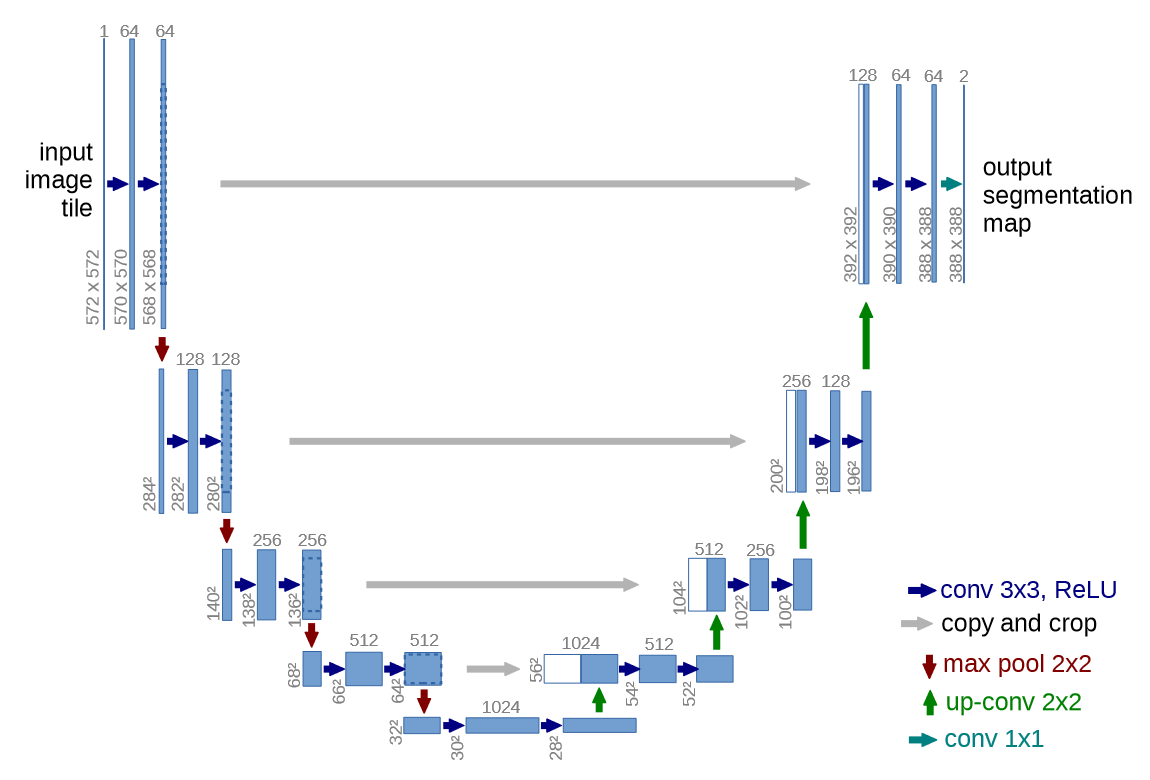
\includegraphics[width=1\linewidth]{media/images/UNet_arch.png}
    \caption{The U-Net architecture with a 2D image of resolution 572$\times$572 as example input. Image reproduced from~\cite{Ronneberger_Fischer_Brox_2015}.}
    \Description[<short description>]{<long description>}
    \label{fig:unet_arch}
\end{figure}

\subsubsection{Attention U-Net}

Attention U-Net extends the original U-Net architecture with the addition of an attention mechanism. This is claimed to improve the sensitivity and prediction accuracy of the network, with minimal impact to the computational cost~\cite{Oktay_2018_AUNet}. The attention mechanism consists of attention gates that filter the features transmitted through the skip connections. This applies additive soft attention to help the network learn to suppress irrelevant features and focus only on the most important features.

In addition to Attention U-Net, several other variants of U-Net have also been proposed in the literature. This includes Residual U-Net~\cite{Zhang_resunet_2018}, Dense U-Net~\cite{Wang_dense_unet_2019}, R2U-Net~\cite{Alom_r2unet_2018}, U-Net++~\cite{Zhou_2018_unet++} and TransUNet~\cite{Chen_transunet_2021}. We chose to test the Attention U-Net with \texttt{peregrine}, since it is the most popular variant (based on the number of article citations at present time), and due to the authors claim that the performance is enhanced without adding additional computational burden.

% U-Net++ replaces the plane skip connections in vanilla U-Net with nested dense skip connections. This is to reduce the semantic gap between the encoder and decoder, which they claim yields significant performance gains.

\subsection{Transformer models}

\subsubsection{Vision Transformer}

Transformer models have revolutionized the field of NLP (Natural Language Processing) with their self-attention mechanisms that do not rely on recurrence or convolutions~\cite{Vaswani_2017_transformer}. Transformer models can also be applied to image recognition tasks, where the image is divided into a sequence of patches. Positional embeddings are combined with the patch embeddings to store the positional information. It has been demonstrated that Vision Transformer models can match, and even outperform state-of-the-art CNN for image classification tasks~\cite{Dosovitskiy_2021_ViT}. The self-attention mechanism of the transformer allows the model to focus on the most relevant parts of the image, which capture the longer-range dependencies more effectively that RNNs or CNNs. Due to the reported high performance of the Vision Transformer over conventional CNN, we would like to test the performance of a Vision Transformer model compared to the U-Net CNN within \texttt{Peregrine}.

The main drawback with transformers in general, is their higher complexity compared to CNNs. This means they require more computational resources (e.g. more RAM, GPUs/TPUs), longer training times and more training data. Pretraining transformers on large amounts of training data to learn general representations, and then fine-tuning them with a smaller amount of task-specific data can be way to achieve high performance using less computational resources~\cite{Tay_Dehghani_Rao_Fedus_Abnar_Chung_Narang_Yogatama_Vaswani_Metzler_2022}.

\subsubsection{Multi-variate Time Series Transformer}

The success of the transformer models in the NLP and computer vision fields, has also attracted great interest in the time-series community~\cite{Wen_Zhou_Zhang_Chen_Ma_Yan_Sun_2023}. Transformers are particularly suited to time series data due to their ability to capture longer-range dependencies. They have been shown to be effective feature extractors in 1D signals~\cite{Nguyen_Miah_Bilodeau_Bouachir_2022}. In ~\cite{Nguyen_Miah_Bilodeau_Bouachir_2022}, the time signal was divided into segments and the encoder part of the traditional transformer used in NLP was used to extract relevant features. The resulting model outperformed state-of-the-art algorithms (in 2022) for detection of Parkinson's disease from signals of a patients gait. 

We have chosen to utilise the multivariate time series (MTS) transformer-based framework proposed for unsupervised representation learning~\cite{Zerveas_2020_mvts}. The authors claim that their approach outperforms all state-of-the-art (as of 2020) supervised methods, by a significant margin, even with limited training data. After pretraining the transformer to extract dense vector representations of the time series through an autoregressive objective, the model can then be applied to downstream tasks such as regression, classification, imputation and forecasting. Due to the claimed performance of this model, we think it is a potential alternative to U-Net. The main difference between the MTS model and the ViT model, is that the MTS has been specifically tailored to focus on sequential patterns, while the ViT focuses on visual features within images.

\subsection{Network pruning}

The attention U-Net and transformers models will increase the complexity compared to the original U-Net that is currently in \texttt{Peregrine}. Even with the potential accuracy increase, the larger networks will place a heavier burden on computational resources and/or require more training data. In order to reduce the number of trainable parameters in the current U-Net, with the intent to decrease the training time, we will investigate whether structural network pruning techniques yield any benefit. Pruning networks has proven itself to be a practical and effective way of compressing networks, as it can help to accelerate inference by removing redundant parameters. Specifically, DepGraph (Dependency Graph), is an automatic method to model residual connections and dependencies between paired layers so groups of parameters can be pruned in a structured way~\cite{Fang_Ma_Song_Mi_Wang_2023}.
